\section{Tradeoff Analysis}
\label{sec:tradeoff}
Disaggregation uncouples the two phases and allows a distinct analysis of the characteristics of each phase, providing valuable insights into the algorithm design. It also expands the design space: now each phase needs to be scaled and scheduled independently based on their latency requirements.

In this section, we analyze the computational pattern of prefill (\S\ref{subsec:analysis_prefill}) and decoding instances (\S\ref{subsec:analysis_decoding}) \emph{post disaggregation}. We aim to identify key parameters and derive guidelines for batching and parallelism in each phase. We then highlight several practical deployment considerations (\S\ref{subsec:practical_problems}). This section lays the foundation for per-gpu goodput optimization.

\subsection{Analysis for Prefill Instance}
\label{subsec:analysis_prefill}

\begin{figure}[!t]
    \centering
    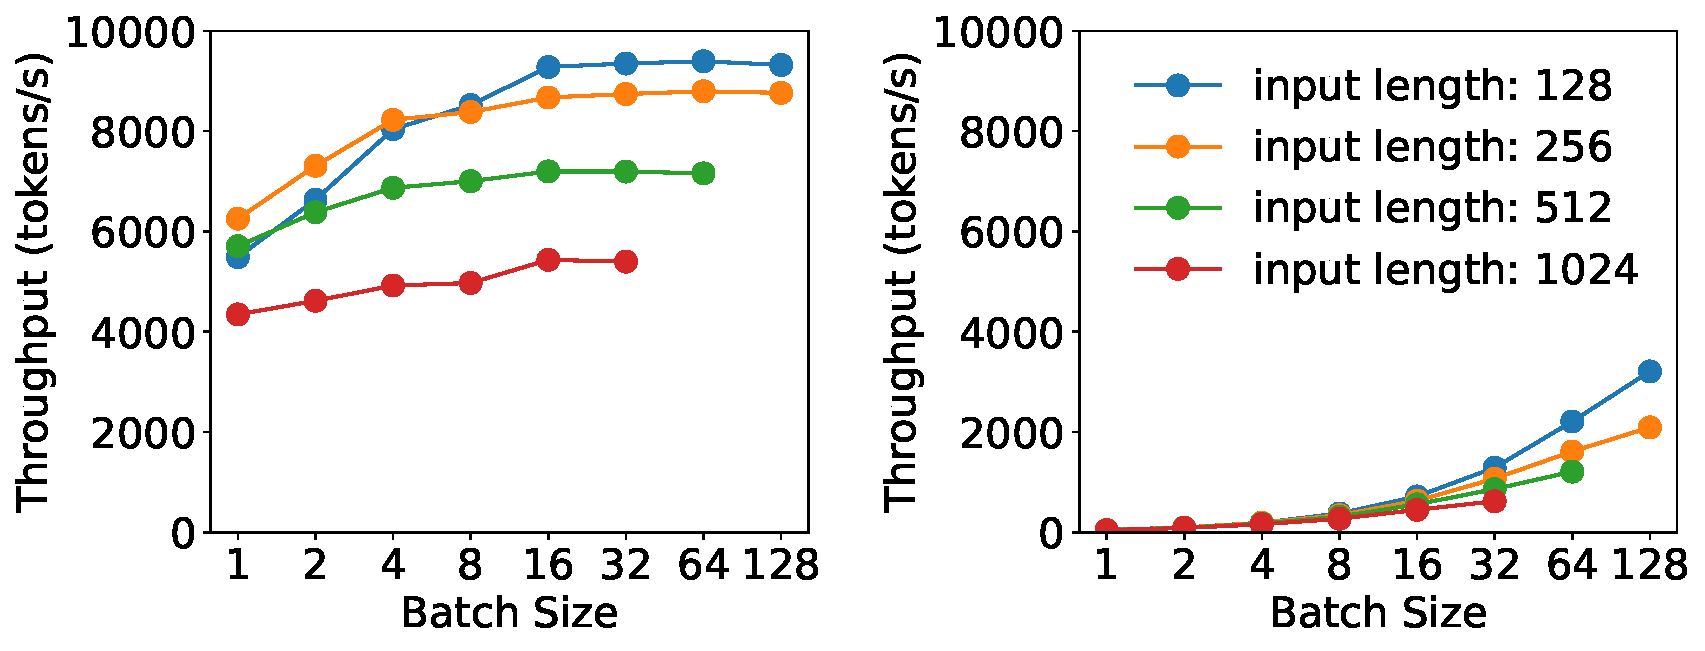
\includegraphics[width=\columnwidth]{figures/prefill_decode_throughput.pdf}
    (a) Prefill phase \hspace{50pt} (b) Decoding phase \hspace{-30pt} 
    \caption{Throughput for two phases with different batch sizes and input lengths when serving an LLM with 13B parameters.}
    \vspace{-4mm}
    \label{fig:prefill_decode_tpt}
\end{figure}

After disaggregation, the prefill phase generates the first token by processing all tokens of the user prompt in parallel. Assuming a given arrival rate, we aim to fulfill the service's latency requirement on TTFT using the least resources.

\parabf{Batching strategy.} The prefill step is typically compute-intensive. Figure~\ref{fig:prefill_decode_tpt}\textcolor{green!80!black}{(a)} shows how the throughput of the prefill phase changes with the input length and the batch size. For a 13B parameter LLM, processing a single sequence of 512 tokens can fully engage an A100 GPU. 
Once the GPU becomes compute-bound, adding more requests to the batch no longer improves GPU efficiency. Instead, it proportionally extends the total processing time for the batch, inadvertently delaying all included requests. Hence, for prefill instances, it is necessary to profile the specific LLM and GPUs in advance to identify a critical input length threshold, denoted as $L_m$, beyond which the prefill phase becomes compute-bound. Batching more requests should only be considered when the input length of the scheduled request is below $L_m$. 
In practice, user prompts typically average over hundreds of tokens~\cite{sharegpt}. Batch sizes for the prefill instance are generally kept small.


\parabf{Parallelism plan.} 
To study the parallelism preferences for prefill-only instances, we serve a 66B LLM on two A100 GPUs with inter-op or intra-op parallelism strategy. To simplify the problem, we assume uniform requests input lengths of 512 tokens and a Poisson arrival process. We compare the resulting average TTFT at various arrival rates in Figure~\ref{fig:prefill_intra_op}\textcolor{green!80!black}{(a)}: intra-op parallelism is more efficient at lower arrival rates, while inter-op parallelism gains superiority as the rate increases.
Disaggregation enables the prefill phase to function analogously to an M/D/1 queue, so we can use queuing theory to verify the observation.

We start by developing notations using the single-device case without parallelism: 
each request's execution time, denoted as $D$, remains constant due to uniform prefill length. Since one request saturates the GPU, we schedule requests via First-Come-First-Served (FCFS) without batching. 
Suppose the Poisson arrival rate is $R$ and the utilization condition of $RD < 1$, the average TTFT ($Avg\_TTFT$) can be modeled by the M/D/1 queue~\cite{shortle2018fundamentals} in close form:
\begin{equation}
\small
    Avg\_TTFT = D + \frac{RD^2}{2(1-RD)}.
    \label{eq1}
\end{equation}
where the first term represents the execution time and the second corresponds to the queuing delay. 
Based on Eq.~\ref{eq1}, we incorporate parallelism below. 

With 2-way inter-op parallelism, we assume the request-level latency becomes $D_s$, and the slowest stage takes $D_m$ to finish. We have $D \approx D_s \approx 2 \times D_m$, due to negligible inter-layer activation communication~\cite{alpa,li2023alpaserve}. The average TTFT with 2-way inter-op parallelism is derived as:

\begin{equation}
\small
    Avg\_TTFT_{inter} = D_s + \frac{RD_m^2}{2(1-RD_m)} = D + \frac{RD^2}{4(2-RD)}.
    \label{eq2}
\end{equation}

For intra-op parallelism, we introduce a speedup coefficient $K$, where $1 < K < 2$, reflecting the imperfect speedup caused by high communication overheads of intra-op parallelism. 
With the execution time $D_s = \frac{D}{K}$, the average TTFT for 2-degree intra-op parallelism is:

\begin{equation}
\small
    Avg\_TTFT_{intra} = \frac{D}{K} + \frac{RD^2}{2K(K-RD)}.
    \label{eq3}
\end{equation}

Comparing Eq.~\ref{eq2} and Eq.~\ref{eq3}: at lower rates, where execution time (first term) is the primary factor, intra-op parallelism's reduction in execution time makes it more efficient. As the rate increases and the queuing delay (second term) becomes more significant, inter-op parallelism becomes advantageous, concurred with Figure~\ref{fig:prefill_intra_op}\textcolor{green!80!black}{(a)}.

The prefill phase's preference for parallelism is also influenced by TTFT SLO and the speedup coefficient $K$. 
Seen from Figure~\ref{fig:prefill_intra_op}\textcolor{green!80!black}{(a)}: A more stringent SLO will make intra-op parallelism more advantageous, due to its ability to reduce execution time.
The value of K depends on factors such as the input length, model architecture, communication bandwidth, and placement~\cite{shoeybi2020megatronlm,alpa}. As shown in Figure~\ref{fig:prefill_intra_op}\textcolor{green!80!black}{(b)}, a decrease in K notably reduces the efficacy of intra-op parallelism.
\S\ref{sec:method} develops algorithms that optimize the resource and parallelism configurations taking into consideration these knobs. 

\begin{figure}[!t]
    \centering
    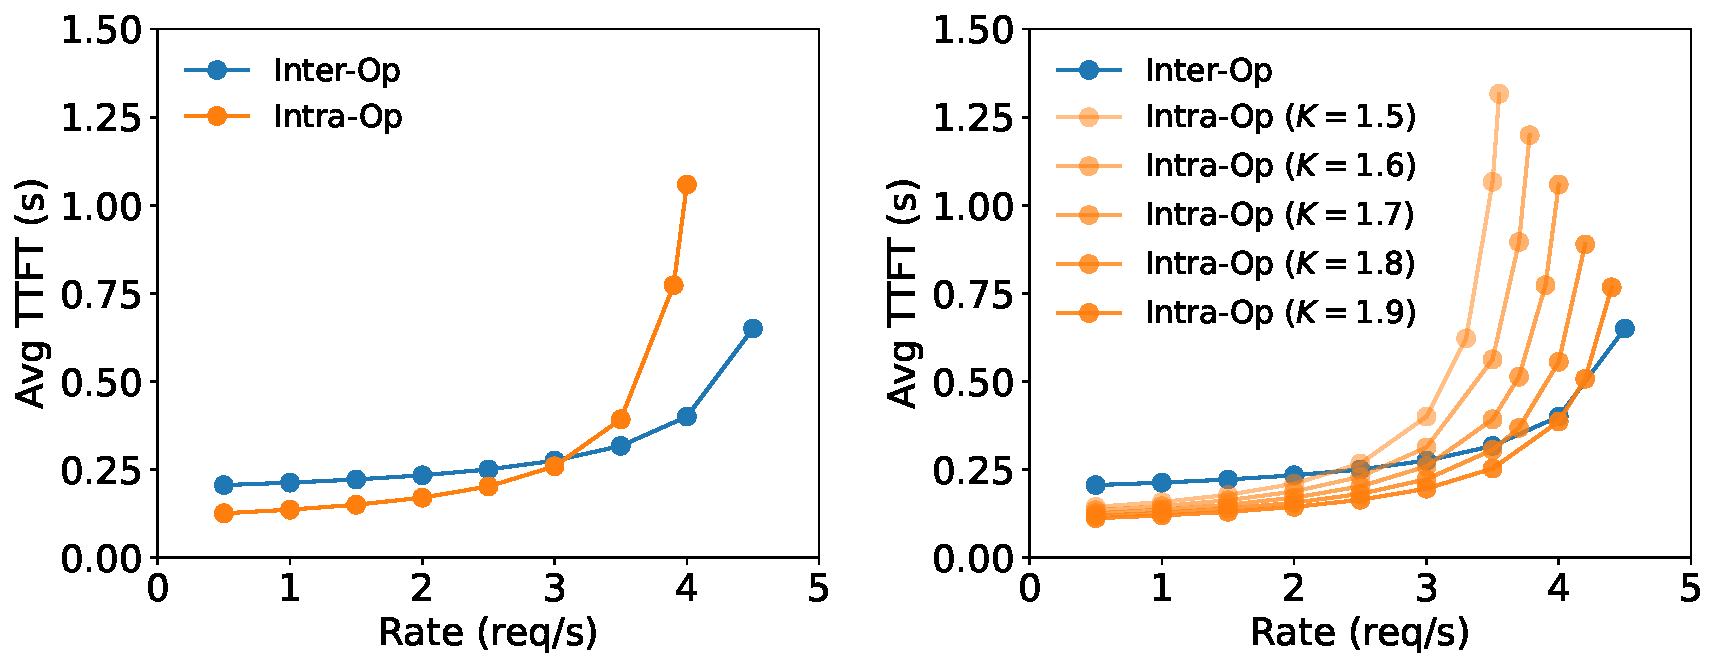
\includegraphics[width=\columnwidth]{figures/prefill_intra_op.pdf}
    (a) Real experiment results \hspace{7pt} (b) Changing intra-op speedup
    \vspace{-0.5mm}
    \caption{Average TTFT when serving an LLM with 66B parameters using different parallelism on two A100 GPUs. }
    \vspace{-4.9mm}
    \label{fig:prefill_intra_op}
\end{figure}


\subsection{Analysis for Decoding Instance}
\label{subsec:analysis_decoding}
Unlike the prefill instance, a decoding instance follows a distinct computational pattern: it receives the KV caches and the first output token from the prefill instance and generates subsequent tokens one at a time. 
For decoding instances, our optimization goal is to satisfy the application's TPOT requirement using minimal computing resources.


\parabf{Batching strategy.} Since a single decoding job is heavily bandwidth-bound, batching is key to avoiding low GPU utilization (hence high per-gpu goodput), as shown in Figure~\ref{fig:prefill_decode_tpt}\textcolor{green!80!black}{(b)}. 
In existing systems where the prefill and decoding phases are colocated, increasing the decoding batch size is difficult because it conflicts with meeting latency goals, particularly in scenarios with high request rates. This is because sharing GPUs cause competition between prefill and decoding jobs, leading to a trade-off between TTFT and TPOT. For example, a higher arrival rate generates more prefill jobs, demanding greater GPU time to meet TTFT requirements if prioritizing prefill jobs, which in turn adversely affects TPOT.

On the contrary, disaggregation offers a solution by enabling the allocation of multiple prefill instances to a single decoding instance. This approach allows for accumulating a larger batch size on dedicated GPUs for the decoding phase without sacrificing TPOT.

\begin{figure}[!t]
    \centering
    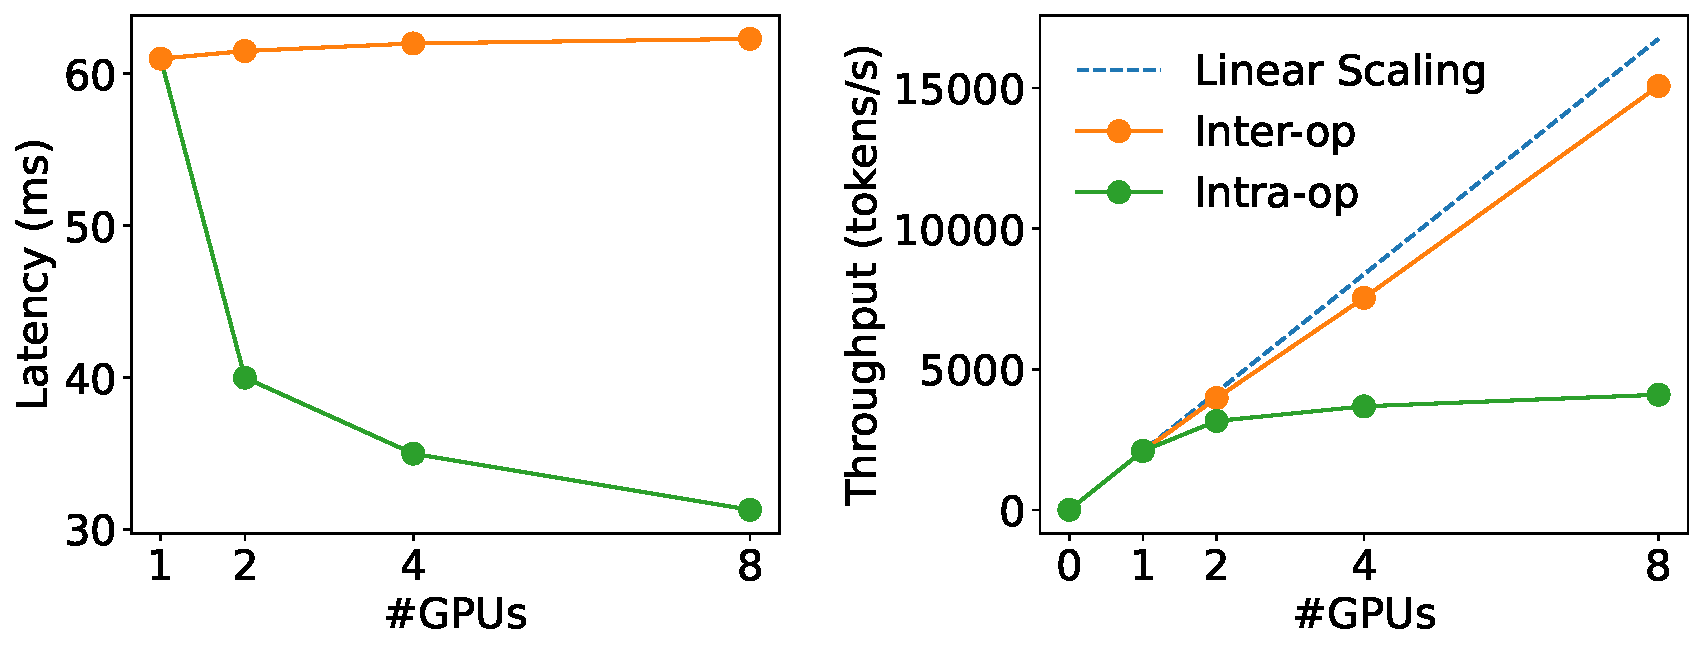
\includegraphics[width=\columnwidth]{figures/decode_parallel.pdf}
    \caption{Decoding phase latency and throughput when serving a 13B LLM with batch size = 128 and input length = 256 under different parallel degrees.}
    \vspace{-4mm}
    \label{fig:decode_parallel}
\end{figure}

\parabf{Parallelism plan.} Post-disaggregation, the batch size for decoding may be constrained by GPU memory capacity, as it is necessary to maintain the KV caches for all active requests.
Scaling the decoding instance with model parallelism or leveraging advanced memory management techniques for LLM KV caches, such as Paged-Attention~\cite{vllm} and GQA~\cite{ainslie2023gqa}, enable further scaling of the decoding batch size to nearly compute-bound. 
As the decoding batch size continue to increase to approach the compute-bound, the decoding computation begins to resemble the prefill phase. With this observation, we investigate how the latency and throughput change under different parallelism degrees under large batch conditions in Figure~\ref{fig:decode_parallel}: intra-op parallelism reduces latency with diminishing returns, caused by communication and reduced utilization after partitioning. Inter-op parallelism can almost linearly scale the throughput. Hence, when the TPOT SLO is stringent, intra-op parallelism is essential to reduce TPOT to meet latency goals. Beyond this, inter-op parallelism is preferable to enhance throughput linearly.

It is worth noting that when the model can fit into the memory of a single GPU, replication is a competitive option in addition to model parallelism for both prefill and decoding instances, to linearly scale the system's rate capacity. It may also reduce the queuing delay -- as indicated by Eq.~\ref{eq1}  -- by substituting $R$ with $R/N$ assuming requests are equally dispatched to $N$ replicas, at the cost of maintaining additional replicas of the model weights in GPU memory.


\subsection{Practical Problems}
\label{subsec:practical_problems}
We have developed foundational principles for selecting batching and parallelisms for each phase. In this section, we discuss and address several challenges encountered during the practical deployment of disaggregated prefill and decoding phases.

\parabf{Variable prefill length.} \S\ref{sec:tradeoff} has assumed uniform prompt length across requests. In real deployments, depending on the LLM application, the lengths of requests are non-uniform. The non-uniformity can cause pipeline bubbles~\cite{huang2019gpipe,pipedream} for prefill instances applying inter-op parallelism because the execution time of pipeline stages across requests of different lengths will vary. This results in slight deviations from the conclusions indicated by using the M/D/1 queue model. To address the problem, \S\ref{sec:method} develops algorithms that search for parallelisms based on workloads, and resort to scheduling to minimize the bubbles (\S\ref{subsec:online_scheduling}).


\parabf{Communication overhead.}
Transferring KV caches from prefill to decoding instances incurs notable overheads. For example, the KV cache size of a single 512-token request on OPT-66B is approximately 1.13GB. Assuming an average arrival rate of 10 rps, we need to transfer 11.3GB data per second---or equivalently 90Gbps bandwidth to render the overhead invisible. While many modern GPU clusters for LLMs are equipped with InfiniBand (e.g., 800 Gbps), in cases where cross-node bandwidth is limited, \sys relies on the commonly available intra-node NVLINK, where the peak bandwidth between A100 GPUs is 600 GB/s, again rendering the transmission overhead negligible (see \S\ref{exp:breakdown}). However, this requirement imposes additional constraints on the placement of prefill and decoding instances that we take into consideration in the next section.


Through the analysis in this section, we identify the workload pattern, placement constraints, SLO requirements, parallelism strategies, and resource allocation as key parameters that create a web of considerations in designing the disaggregated serving system. How to automatically navigate the search space to find the configuration that achieves optimal per-gpu goodput is challenging, and addressed next.
